% Management Summary

\begingroup
\let\clearpage\relax
\let\cleardoublepage\relax
\let\cleardoublepage\relax

\chapter*{Management Summary}
\label{management-summary}

\subsection*{Situation}\label{introduction}

Web mapping has gone through different technological changes in recent years. 
After serving static images for an extract of the map, Google introduced raster tile based maps with Google Maps and it soon became the standard for web maps.\\
Now the major players have shifted to using vector tiles. Vector tiles allow map designers to individually design their own map. The system administrator does not need to manage large infrastructure, as the tile rendering process can be offloaded to the client side. This results in faster maps with a better user experience.
\begin{figure}[H]
  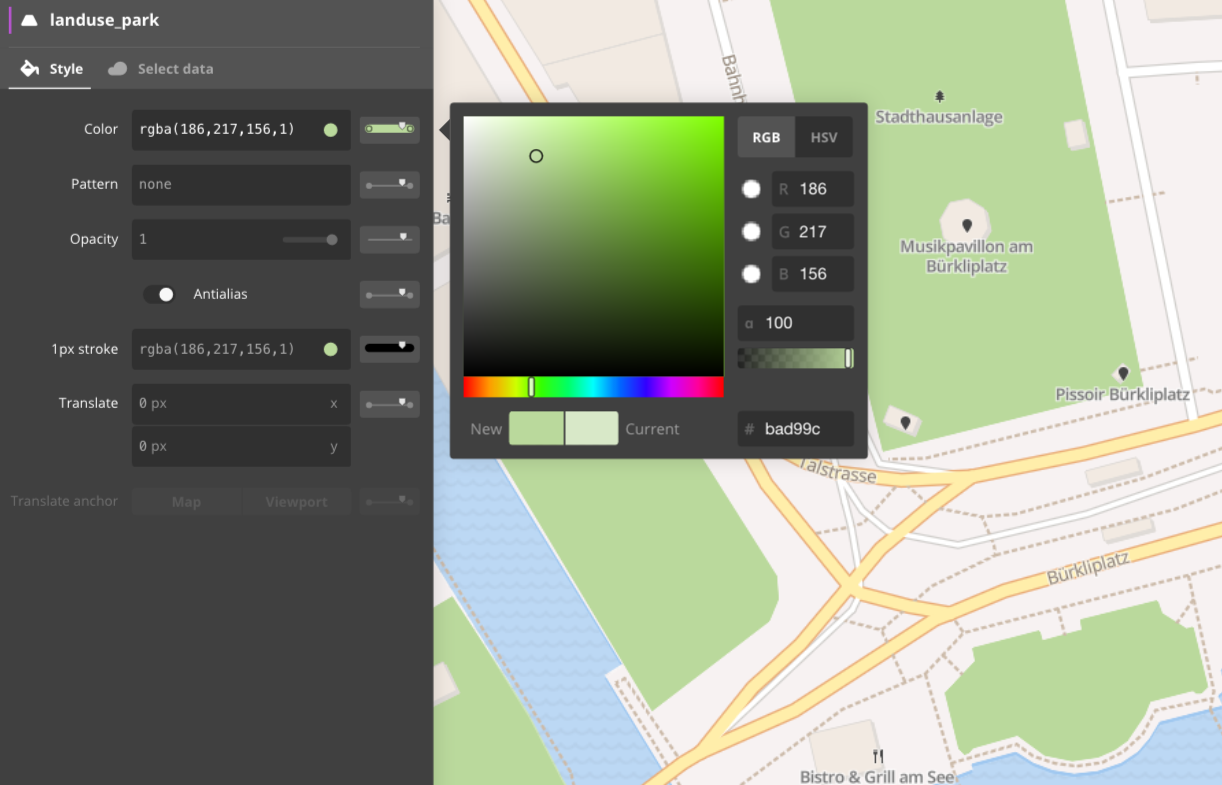
\includegraphics[width=1\textwidth]{images/custom_map.png}
  \caption{Custom styling of maps in Mapbox Studio}
\end{figure}
A few existing providers opened the process of creating vector tiles, but still own the data to promote their services. Producing vector tiles requires a good understanding of map technologies and sufficient computing power. This is the reason, why vector tiles aren't adopted by the main stream yet.

\subsection*{Approach}

The main objective of this project is to create free and open-source vector tiles of Open Street Map data. So that every developer, cartographer or designer can create their custom maps.\\ 
An entire workflow for producing vector tiles was defined and a vector tile server to serve the produced vector tiles was implemented. The vector tiles are compatible with the vector tiles of Mapbox Streets, therefore the same visual style provided by Mapbox can be used with our vector tiles. The figure below shows the Mapbox Artistic Woodcut visual style, which can be used with our vector tiles as data source.

\begin{figure}[H]
  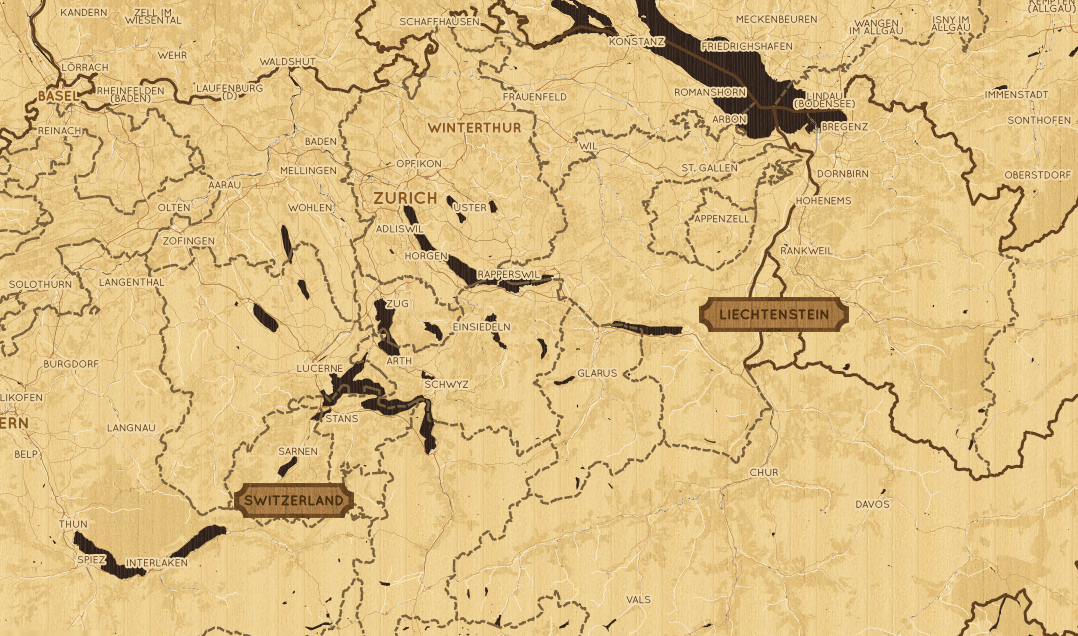
\includegraphics[width=1\textwidth]{images/woodcut.png}
  \caption{Mapbox's Artistic Woodcut visual style}
\end{figure}


\subsection*{Result}
The result of this thesis are vector tiles of Switzerland. They are available for download from the project website(\url{http://osm2vectortiles.org}). These vector tiles can be served together with a custom or Mapbox visual style in our vector tile server.\\
As the entire workflow of creating vector tiles is documented and open-source available, other organizations could now use this project to produce vector tiles of their own datasets.
\endgroup

\vfill
